\documentclass[a4paper]{article}
\usepackage{graphicx}
\usepackage{amsmath}
\usepackage{amsmath}
\usepackage{geometry}
 \geometry{
 a4paper,
 total={150mm,257mm},
 top=20mm,
 }
\begin{document}
\begin{figure}
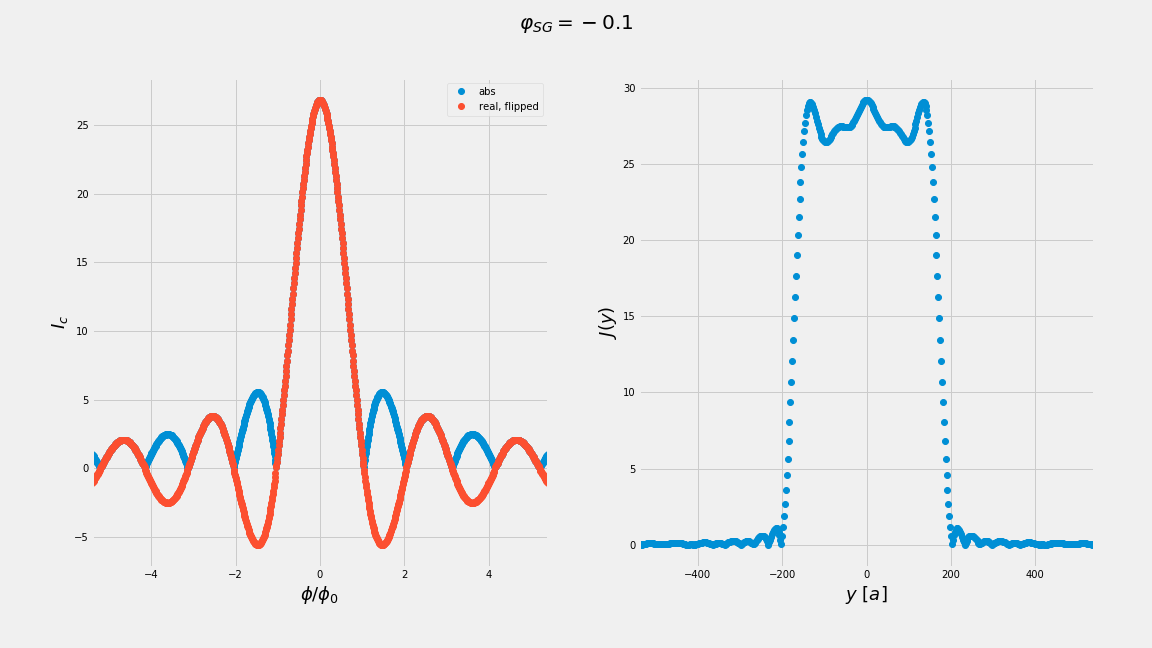
\includegraphics[width=\textwidth]{figs/wg32double/current_and_density_01}
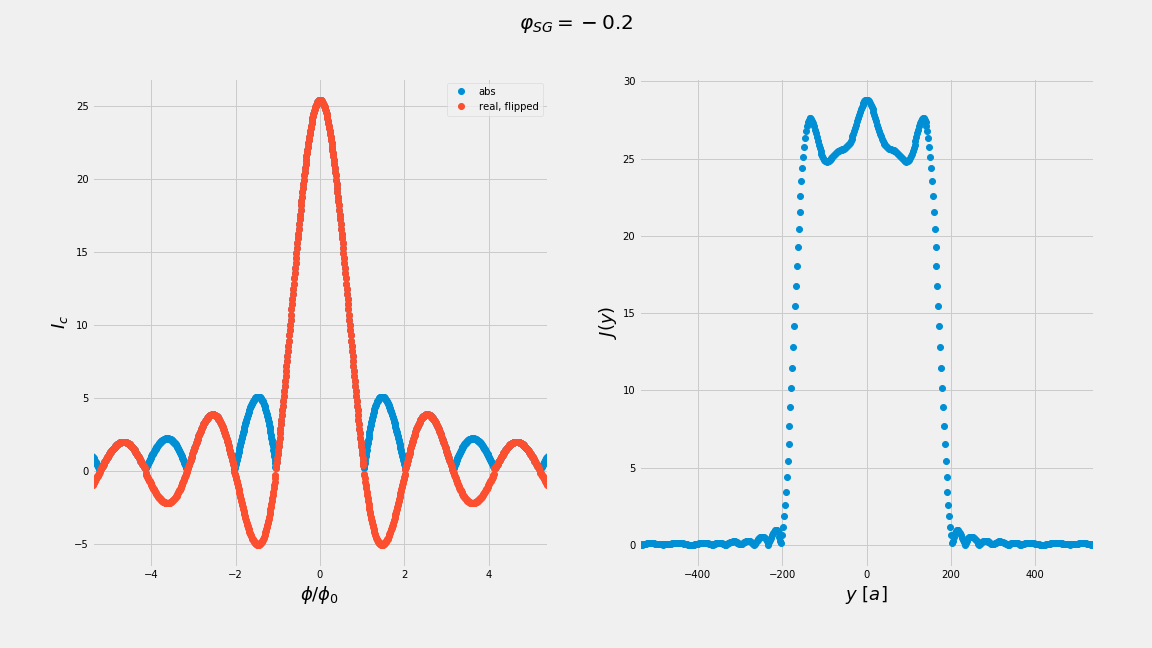
\includegraphics[width=\textwidth]{figs/wg32double/current_and_density_02}
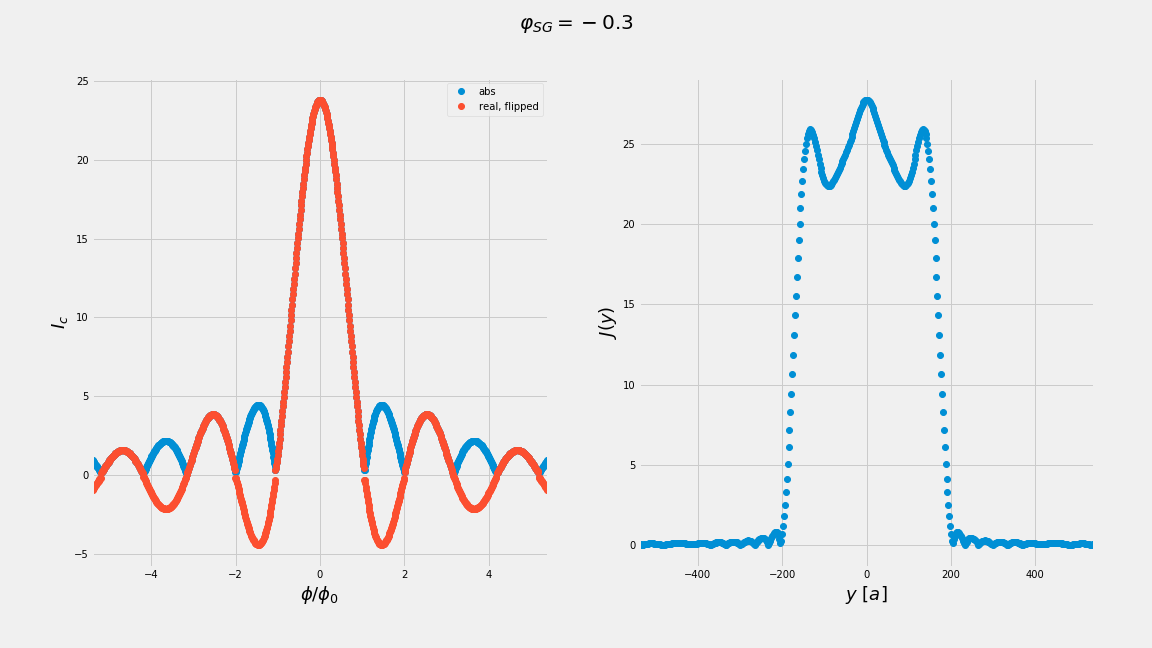
\includegraphics[width=\textwidth]{figs/wg32double/current_and_density_03}
\end{figure}
\begin{figure}
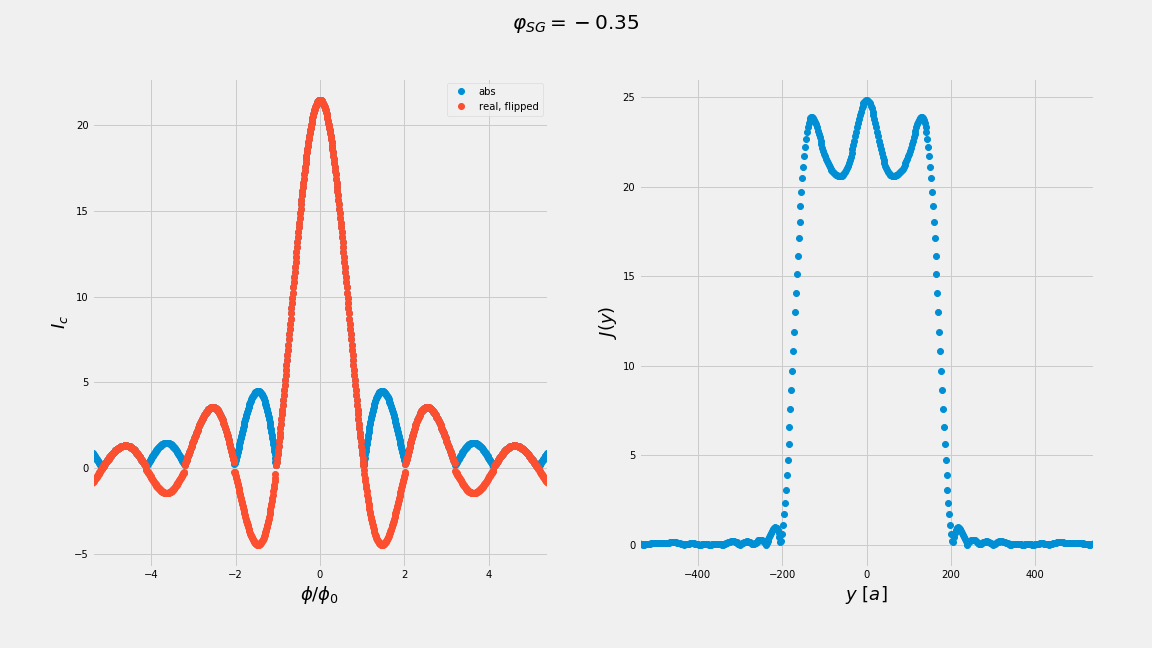
\includegraphics[width=\textwidth]{figs/wg32double/current_and_density_035}
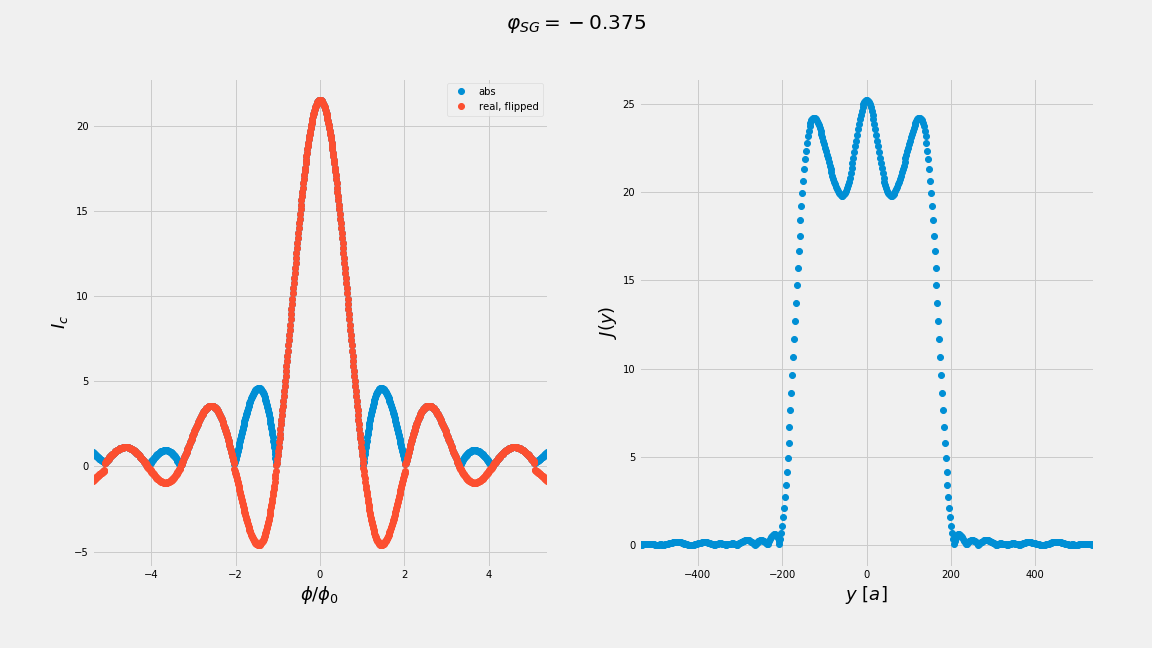
\includegraphics[width=\textwidth]{figs/wg32double/current_and_density_0375}
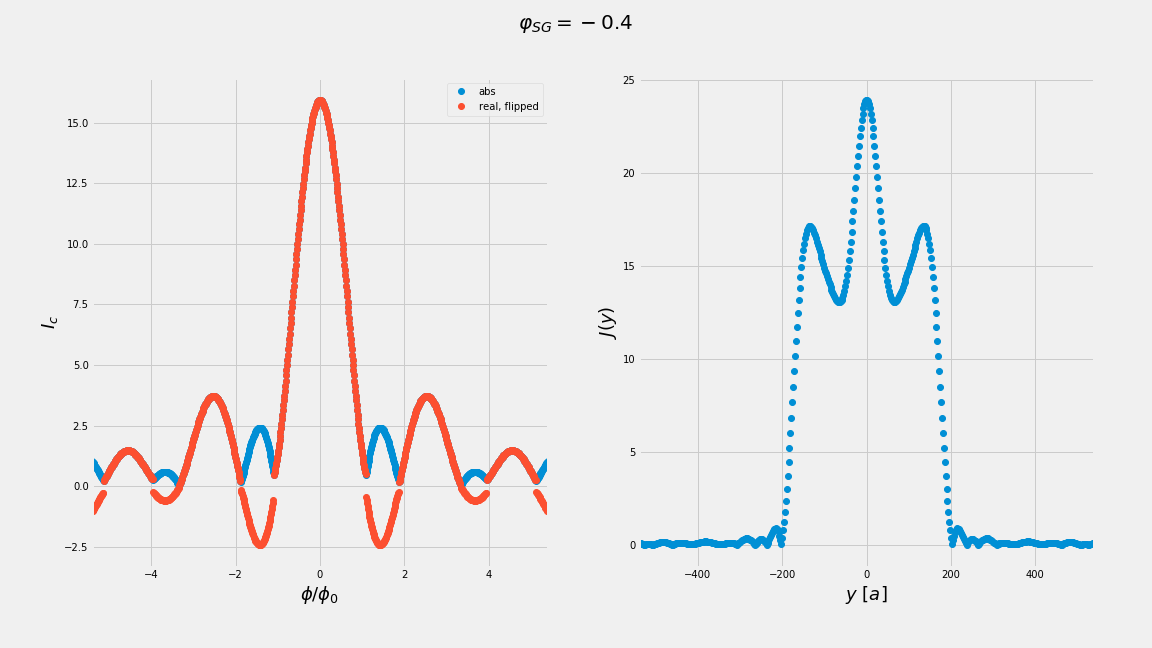
\includegraphics[width=\textwidth]{figs/wg32double/current_and_density_04}
\end{figure}
\begin{figure}
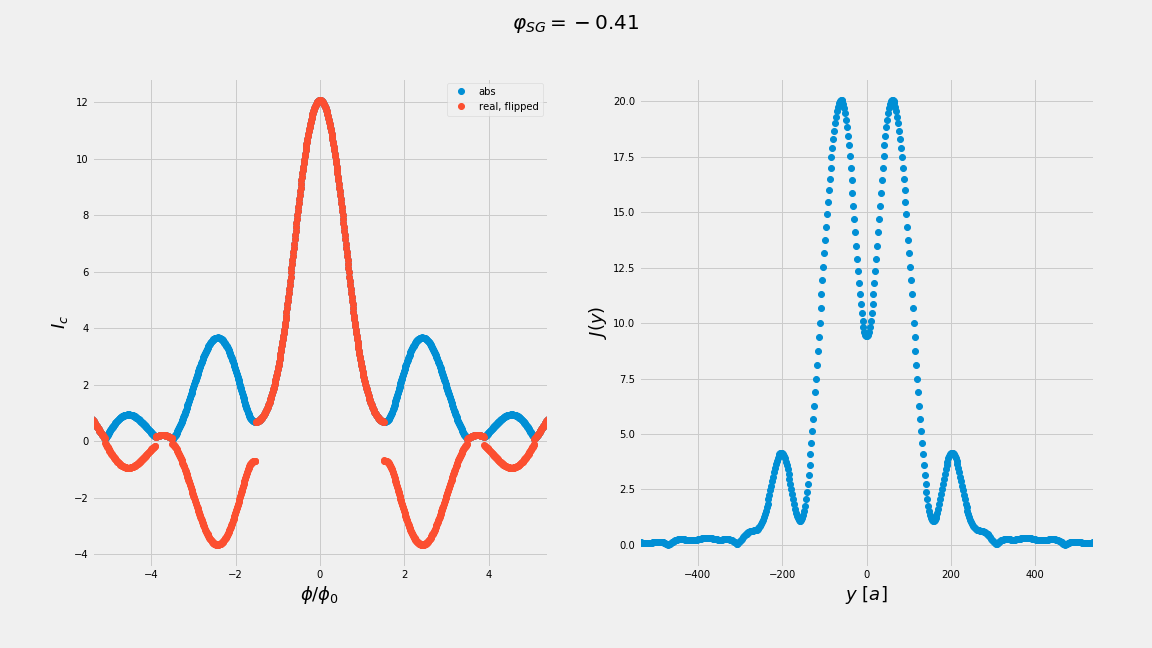
\includegraphics[width=\textwidth]{figs/wg32double/current_and_density_041}
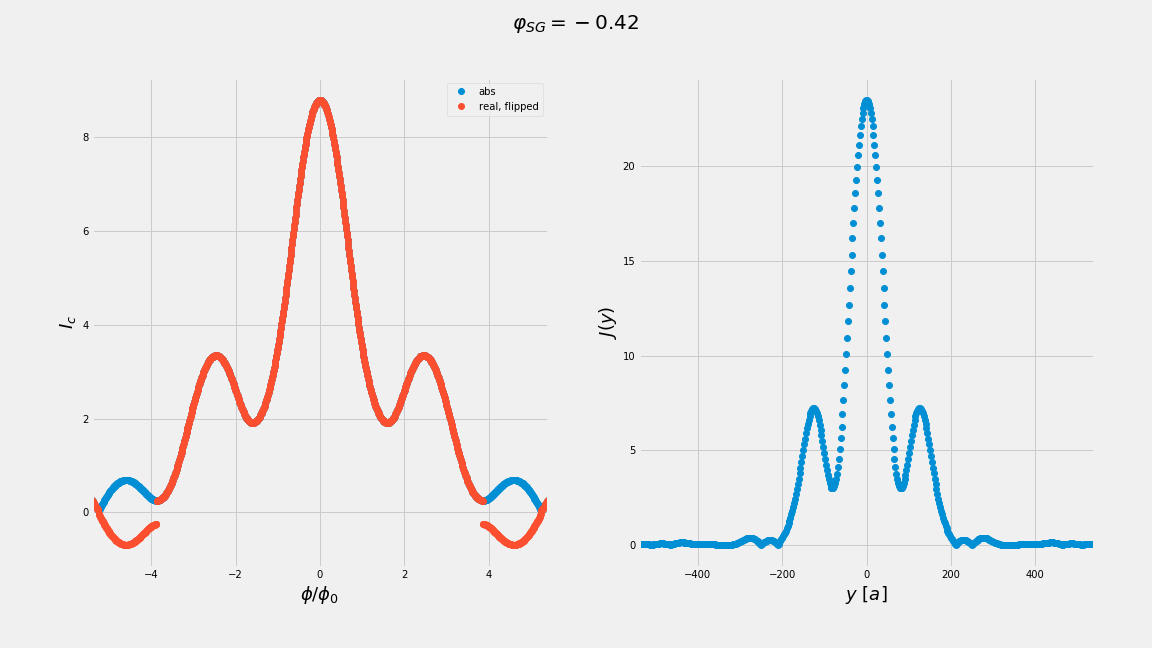
\includegraphics[width=\textwidth]{figs/wg32double/current_and_density_042}
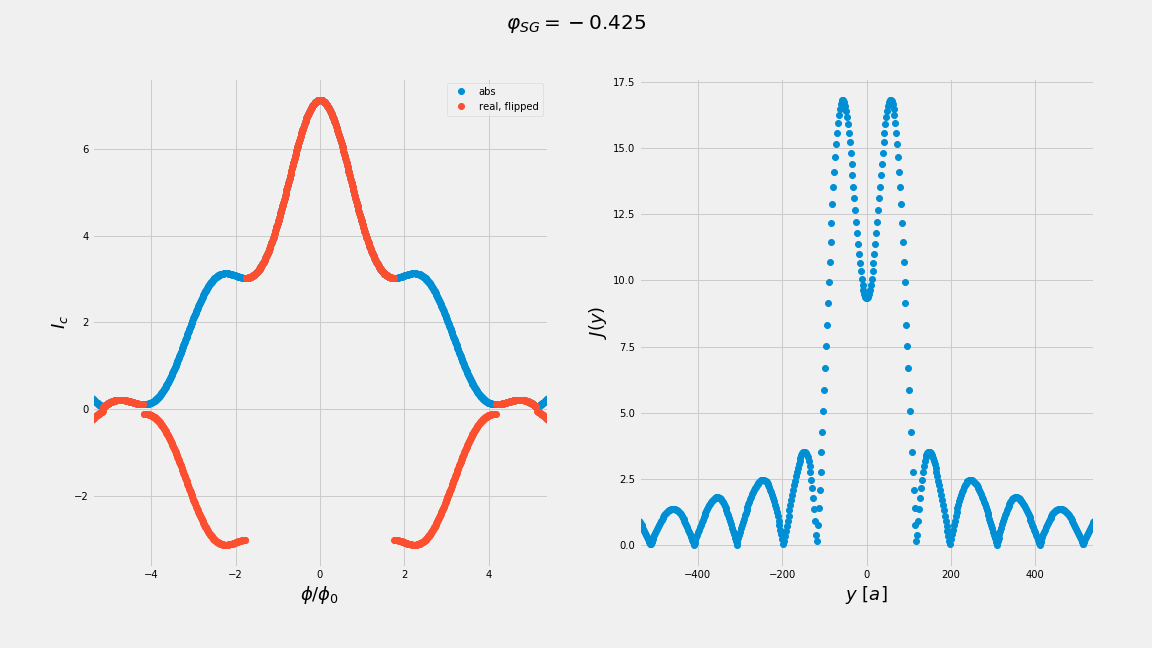
\includegraphics[width=\textwidth]{figs/wg32double/current_and_density_0425}
\end{figure}
\begin{figure}
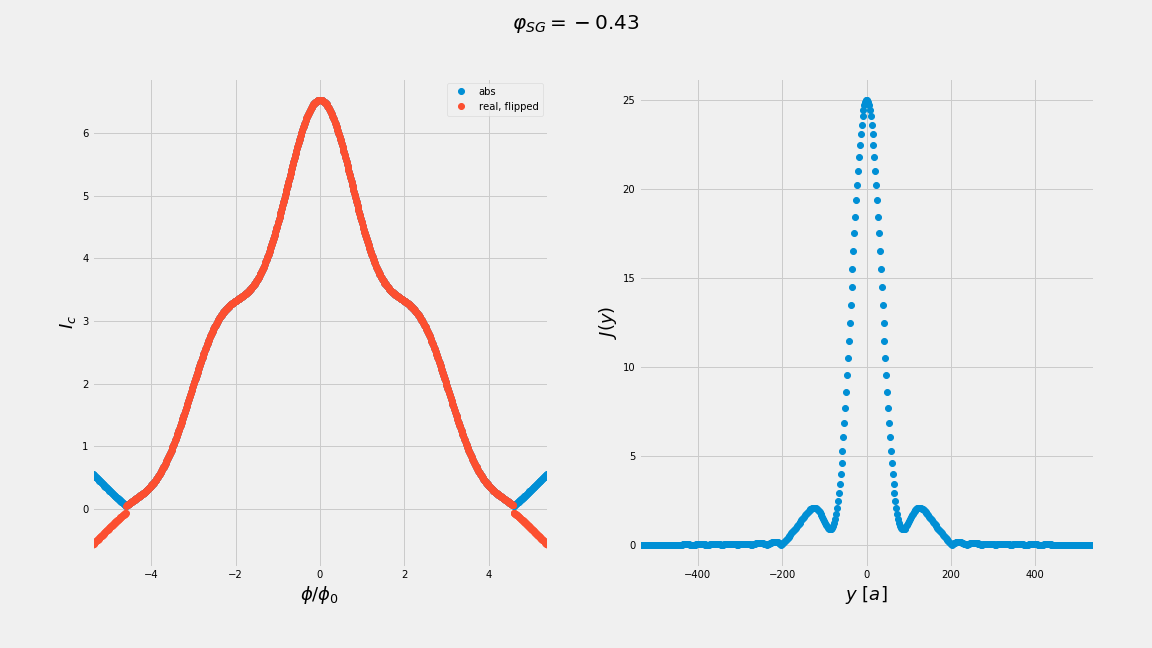
\includegraphics[width=\textwidth]{figs/wg32double/current_and_density_043}
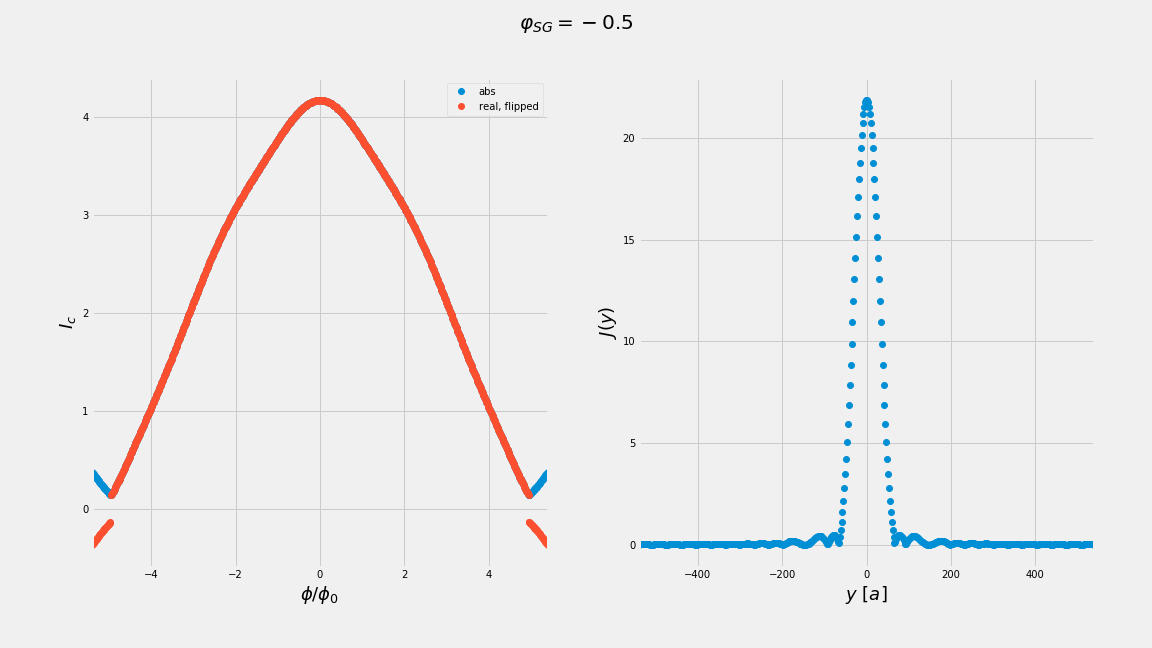
\includegraphics[width=\textwidth]{figs/wg32double/current_and_density_05}
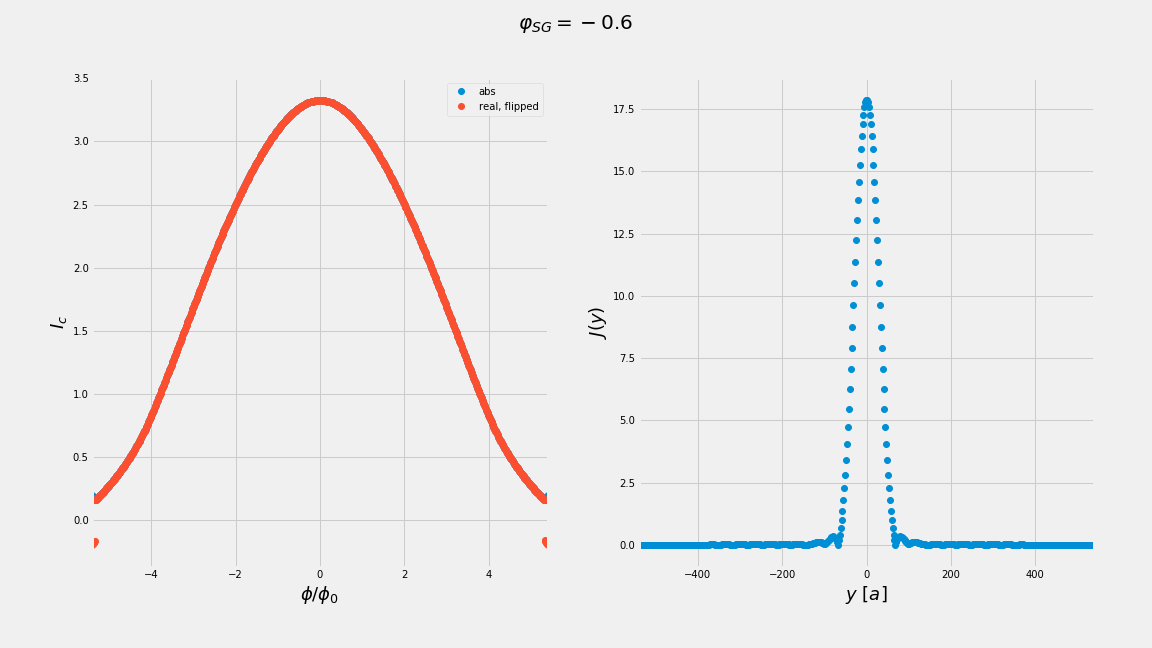
\includegraphics[width=\textwidth]{figs/wg32double/current_and_density_06}
\end{figure}
\end{document}